\chapter{Założenia projektowe}

Tematem pracy jest stworzenie aplikacji wspomagającej szacowanie historyjek metodą Planning Poker.
Aplikacja pozwoli na przeprowadzenie gry, której backlog będzie pochodził z serwisu Github,
a wyniki gry będą zapisywane jako etykiety opisujące poszczególne zadania w Github.

Aplikacja będzie synchronizowana z Githubem,
czyli że jeżeli jakieś zadanie będzie z niego usunięte, usunięte zostanie również
z aplikacji.

Gra będzie posiadała także możliwości zamknięcia danego zadanie oraz jego edycji.

Inną planowaną funkcją jest możliwość tworzenia własnej skali estymacji.

Gracze będą dodawani do gry przez dzielenie się linkiem,
jednakże właściciel będzie mógł gracza wyrzucić z gry.

\section{Wymagania funkcjonalne}

\begin{itemize}
    \item Logowanie przez Github
    \item Logowanie jako gość (anonimowe)
    \item Pobieranie historyjek z Github
    \item Synchronizacja z Github
    \item Możliwość tworzenia list z issues Github
    \item Możliwość tworzenia gry
    \item Możliwość zapraszania graczy
    \item Możliwość głosowania przez graczy
    \item Możliwość tworzenia własnej skali estymacji
    \item Możliwość komentowania każdej historyjki podczas gry
    \item Możliwość automatycznego przeliczania wyników
    \item Możliwość wyrzucenia gracza z gry przez właściciela
    \item Możliwość eksportu wyników gry w postaci historyjek do Github
\end{itemize}

\section{Wymagania niefunkcjonalne}

\begin{itemize}
    \item Oprogramowanie musi być responsywne i proste.
    \item Aplikacja powinna się uruchamiać w przeglądarce internetowej.
    \item Aplikacja powinna działać w najnowszych wersjach przeglądarek.
    \item Aplikacja powinna działać w czasie rzeczywistym.
    \item Serwer powinien obsłużyć co najmniej 200 połączeń użytkowników.
    \item Zapewnienie bezpieczeństwa danych.
\end{itemize}

\section{Sposób komunikacji}

Aby aplikacja mogła komunikować się w czasie rzeczywistym niezbędne jest wykorzystanie
protokołu Websockets (patrz rysunek \ref{rys:websocket}).

\begin{figure}[H]
	\centering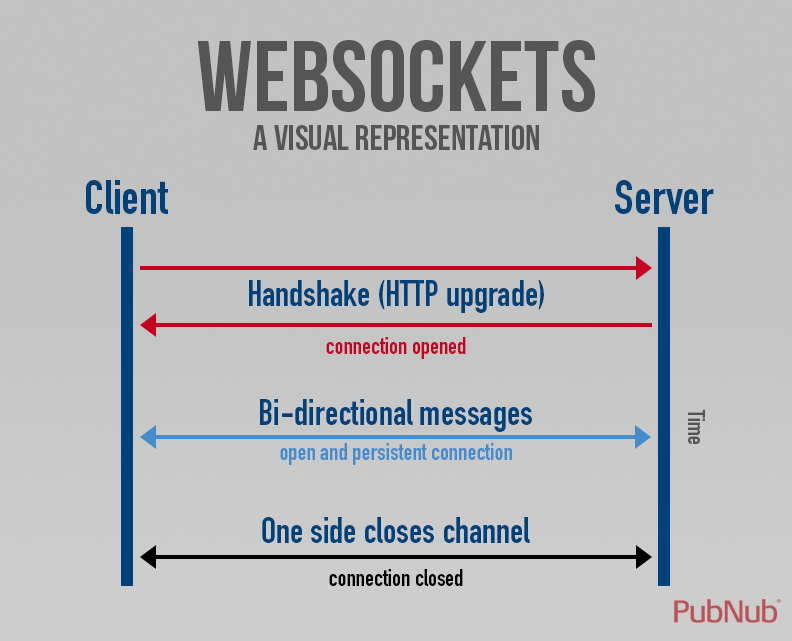
\includegraphics[width=.6\textwidth]{img/websocket}
	\caption{websockets}.
	\label{rys:websocket}
\end{figure}

\section{Wykorzystanie technologie}

Aplikacja zostanie napisana w języku EcmaScript 6, kompilowanego do JavaScript
z wykorzystaniem SCSS, JSX i HTML5.

Wybrany zestaw technologii:
\begin{itemize}
    \item Node.js - środowisko uruchomieniowe do tworzenia aplikacji
    \item Yarn - Manadżer pakietów
    \item React -  biblioteka do tworzenia interfejsu użytkownika
    \item Redux - biblioteka wspomagająca zarządzanie stanem aplikacji
    \item Bootstrap - framework SCSS do budowania responsywnych stron internetowych
    \item Webpack - narzędzie do opakowywania, kompilowania i minimalizowania kodu
    \item Firebase - platforma służąca jako backend aplikacji
\end{itemize}
